%! TEX root = .
\documentclass[a4paper,11pt]{article}

% ====================
% PACKAGES DE BASE
% ====================
\usepackage[utf8]{inputenc}
\usepackage[T1]{fontenc}
\usepackage[french]{babel}
\usepackage{amsmath, amssymb, amsfonts}
\usepackage{graphicx}
\usepackage{geometry}
\usepackage{hyperref}
\usepackage{booktabs}
\usepackage{float}
\usepackage{xcolor}
\usepackage{caption}
\usepackage{subcaption}
\usepackage{siunitx}

% ====================
% MISE EN PAGE
% ====================
\geometry{margin=2.5cm}
\setlength{\parskip}{6pt}
\setlength{\parindent}{0pt}
\hypersetup{
    colorlinks=true,
    linkcolor=blue,
    urlcolor=blue,
    citecolor=blue
}

% ====================
% INFORMATIONS DU DOCUMENT
% ====================
\title{\textbf{Compte rendu du TP4}\\[4pt]
\large Exploitation durable de la forêt}
\author{Groupe : \textit{Maël Verbois, Jules Onnée, Rayen Selmi} \\[2pt] Cours : ROB}


% ====================
% DOCUMENT
% ====================
\begin{document}

\maketitle

\section{Compte Rendu}
% ===========================
L’objectif de ce travail pratique est d’étudier un problème d’optimisation combinatoire inspiré de la gestion durable d’une forêt. 
L’exploitation forestière doit être planifiée de manière à préserver deux espèces animales dont les habitats dépendent des parcelles coupées ou conservées. 
Ce TP vise à formuler ce problème sous forme d’un programme linéaire en variables mixtes, puis à en proposer une version quadratique et sa linéarisation totale. 
Nous comparerons ensuite les performances des différentes approches sur plusieurs instances et analyserons l’impact de contraintes supplémentaires sur la structure du problème.

% ===========================
\section{Formulation du modèle initial (P1)}
% ===========================
\subsection{Présentation du modèle}
% → Ici, tu pourras insérer la formulation mathématique de (P1) en environnement align ou cases
% Exemple :


\[
\begin{aligned}
\max_{x,d} \quad & w_1 \sum_{(i,j)\in M\times N} t_{ij}(1 - x_{ij}) + w_2 g l \sum_{(i,j)\in M\times N} (4x_{ij} - d_{ij}) \\
\text{sous contraintes} \quad &
\begin{cases}
d_{ij} \ge \sum_{(k,l)\in A_{ij}} x_{kl} - |A_{ij}|(1 - x_{ij}) \quad \forall (i,j)\in M\times N,\\[8pt]
d_{ij} \ge 0, \quad x_{ij}\in \{0,1\}
\end{cases}
\end{aligned}
\]

\subsection{Interprétation des variables et paramètres}

\begin{itemize}
    \item $M$ et $N$ : dimension de la matrice représentant la forêt
    \item \item $A_{ij}$ : ensemble des indices $(k,l)$ correspondant aux parcelles adjacentes à $(i,j)$ dans la matrice $M \times N$.
    \item $g$ : population attendue de l'espèce $e_2$ par kilomètre de lisière.
    \item $l$ : longueur du côté d’une parcelle carrée.
    \item $x_{ij} \in \{0,1\}$ : variable binaire associée à la parcelle $(i,j)$
    \begin{itemize}
        \item $x_{ij} = 1$ si la parcelle $(i,j)$ est \textbf{non coupée}
        \item $x_{ij} = 0$ si la parcelle $(i,j)$ est \textbf{coupée}
    \end{itemize}

    \item {$d_{ij} \ge 0$ : variable continue valant à l'optimum:
    
    \begin{itemize}
    \item $0$ si la parcelle $x_{ij}$ est coupée $(x_{ij} = 0)$ car le terme $|A_{ij}|(1-x_{ij})$ désactive la contrainte
    \item $\sum_{(k,l)\in A_{ij}} x_{kl}$ sinon soit le nombre de côtés de la parcelle $s_{ij}$ qui sont adjacents à des parcelles non coupées 
    \end{itemize} 
    
    Tout cela garantit bien que dans l'objectif les termes $(4x_{ij} - d_{ij})$ représentent le nombre de côtés étant une lisière pour les parcelles $(s_{ij})$ et donc 
    $g l \sum_{(i,j)\in M\times N} (4x_{ij} - d_{ij})$ est la population attendue de l'espèce 2}
    \item $t_{ij} \ge 0$ : population attendue de l'espèce $e_1$ dans la parcelle $(i,j)$ si elle est coupée.
    Donc $\sum_{(i,j)\in M\times N} t_{ij}(1 - x_{ij})$ est la population attendue le l'espèce 1
    \item $w_1, w_2$ : coefficients de pondération correspondant à l’importance relative des deux espèces dans la fonction objectif.
\end{itemize}

% ===========================
\section{Programme quadratique (P2)}
Pour passer du programme linéaire en variables mixtes (P1) à un programme quadratique en variables binaires, on peut se passer des variables continues $d_{ij}$.

\subsection{Idée principale}

On remarque que l'interface entre deux parcelles $s_{ij}$ et $s_{kl}$ avec $(k,l)\in A_{ij}$ constitue une \textbf{lisière} pour $s_{ij}$ si et seulement si :
\[
x_{ij} = 1 \quad \text{et} \quad x_{kl} = 0.
\]

Autrement dit, le produit
\[
x_{ij} \cdot (1 - x_{kl})
\]
vaut 1 si cette interface est une lisière pour $s_{ij}$, et 0 sinon.

---

\subsection{Formulation du programme quadratique}

On remplace donc tous les termes de la forme $4x_{ij} - d_{ij}$ dans (P1) par :
\[
\sum_{(k,l) \in A_{ij}} x_{ij} \cdot (1 - x_{kl}),
\]
et on supprime les contraintes sur $d_{ij}$.  

Le programme quadratique obtenu, noté (P2), s'écrit alors :

\begin{align*}
\text{(P2)} \quad 
\max_{x} \quad & w_1 \sum_{(i,j)\in M\times N} t_{ij}(1 - x_{ij}) 
+ w_2 g \, l \sum_{(i,j)\in M\times N} \sum_{(k,l)\in A_{ij}} x_{ij} (1 - x_{kl}) \\
\text{s.c.} \quad & x_{ij} \in \{0,1\} \quad \forall (i,j)\in M\times N.
\end{align*}

\section{Linéarisation du programme (P2)}

\subsection{Développement des produits dans l'objectif}

Dans (P2), la contribution de l'espèce $e_2$ est donnée par :
\[
\sum_{(i,j)\in M\times N} \sum_{(k,l)\in A_{ij}} x_{ij} (1 - x_{kl}).
\]

On peut réécrire chaque terme comme suit :
\[
x_{ij} (1 - x_{kl}) = x_{ij} - x_{ij} x_{kl}.
\]

Ainsi, la somme associée à la population de l'espèce $e_2$ devient :
\[
\sum_{(i,j)\in M\times N} \sum_{(k,l)\in A_{ij}} x_{ij} (1 - x_{kl}) 
= \sum_{(i,j)\in M\times N} \sum_{(k,l)\in A_{ij}} x_{ij} - \sum_{(i,j)\in M\times N} \sum_{(k,l)\in A_{ij}} x_{ij} x_{kl}.
\]

On remarque que :
\[
\sum_{(k,l)\in A_{ij}} x_{ij} = |A_{ij}| x_{ij}.
\]

On obtient donc :
\[
\sum_{(i,j)\in M\times N} \sum_{(k,l)\in A_{ij}} x_{ij} (1 - x_{kl}) 
= \sum_{(i,j)\in M\times N} |A_{ij}| x_{ij} - \sum_{(i,j)\in M\times N} \sum_{(k,l)\in A_{ij}} x_{ij} x_{kl}.
\]

---

\subsection{Introduction des variables de linéarisation}

Pour linéariser le produit $x_{ij} x_{kl}$, on introduit des variables binaires :
\[
y_{ijkl} := x_{ij} x_{kl}, \quad \forall (i,j)\in M\times N, \, (k,l)\in A_{ij}.
\]

Le programme linéarisé équivalent devient alors :

\begin{align*}
\max \quad & w_1 \sum_{(i,j)\in M\times N} t_{ij} (1 - x_{ij}) 
+ w_2 g l \sum_{(i,j)\in M\times N} \Big( |A_{ij}| x_{ij} - \sum_{(k,l)\in A_{ij}} y_{ijkl} \Big) \\
\text{s.c.} \quad 
& y_{ijkl} \le x_{ij}, \quad \forall (i,j),(k,l) \\
& y_{ijkl} \le x_{kl}, \quad \forall (i,j),(k,l) \\
& y_{ijkl} \ge x_{ij} + x_{kl} - 1, \quad \forall (i,j),(k,l) \\
& y_{ijkl} \ge 0, \quad x_{ij} \in \{0,1\}, \quad \forall (i,j),(k,l)
\end{align*}

\subsection{Simplification des contraintes}

Comme il s'agit d'un problème de maximisation et que les coefficients associés aux $y_{ijkl}$ sont négatifs dans la fonction objectif, seules les deux dernières contraintes sont actives à l'optimum. On peut donc simplifier le modèle linéarisé :

\begin{align*}
\max \quad & w_1 \sum_{(i,j)\in M\times N} t_{ij} (1 - x_{ij}) 
+ w_2 g l \sum_{(i,j)\in M\times N} \Big( |A_{ij}| x_{ij} - \sum_{(k,l)\in A_{ij}} y_{ijkl} \Big) \\
\text{s.c.} \quad 
& y_{ijkl} \ge x_{ij} + x_{kl} - 1, \quad \forall (i,j),(k,l) \\
& y_{ijkl} \ge 0, \quad x_{ij} \in \{0,1\}, \quad \forall (i,j),(k,l)
\end{align*}

Par un raisonnement par l'absurde, supposons qu'à l'optimum une variable \(y_{ijkl} > 1\).  
Dans ce cas, comme le coefficient associé à \(y_{ijkl}\) dans la fonction objectif est négatif, on pourrait diminuer \(y_{ijkl}\) jusqu’à \(1\) sans violer aucune contrainte tout en augmentant la valeur de l’objectif.  
Ceci contredit l’optimalité.  
Ainsi, à l’optimum on a nécessairement \(y_{ijkl} \le 1\).  

On peut donc ajouter la contrainte :
\[
y_{ijkl} \le 1
\]
et par disjonction de cas sur les valeurs possibles de $x_{ij}$, $x_{kl}$ on a \(y_{ijkl} \in \{0,1\}\), sans modifier la valeur optimale du problème.

\subsection{Modèle final}
\begin{align*}
\max \quad & w_1 \sum_{(i,j)\in M\times N} t_{ij} (1 - x_{ij}) 
+ w_2 g l \sum_{(i,j)\in M\times N} \Big( |A_{ij}| x_{ij} - \sum_{(k,l)\in A_{ij}} y_{ijkl} \Big) \\
\text{s.c.} \quad 
& y_{ijkl} \ge x_{ij} + x_{kl} - 1, \quad \forall (i,j),(k,l) \\
& y_{ijkl} \in \{0,1\} , \quad x_{ij} \in \{0,1\}, \quad \forall (i,j),(k,l)
\end{align*}
\subsection{Preuve de la totale unimodularité}


Pour étudier la structure de la matrice des contraintes, on relâche les contraintes d’intégrité sur les variables \(x_{ij}\) et \(y_{ijkl}\).  
Le programme devient donc un programme linéaire dont les contraintes s’écrivent sous trois formes distinctes :
\begin{align*}
\text{(i)} &\quad x_{ij} + x_{kl} - y_{ijkl} \le 1, \\
\text{(ii)} &\quad x_{ij} \le 1, \\
\text{(iii)} &\quad y_{ijkl} \le 1.
\end{align*}

\subsection{Structure matricielle du système}

En ordonnant les variables sous la forme d’un vecteur
\[
(x_{ij}) \, | \, (y_{ijkl}),
\]
et en plaçant les contraintes dans l’ordre (i), puis (ii) et (iii) (tout en conservant le même ordre pour les lignes de type (ii) et (iii) que celui du vecteur de variables), on obtient une matrice des contraintes par blocs, que l’on peut écrire schématiquement sous la forme :
\[
\begin{pmatrix}
A & -I \\
I & 0 \\
0 & I
\end{pmatrix},
\]
où :
\begin{itemize}
  \item \(A\) est la matrice d’incidence \emph{sommets–arêtes} d’un graphe en grille représentant les adjacences entre parcelles ;
  \item \(I\) désigne une matrice identité de taille appropriée.
\end{itemize}

Comme le graphe de grille est biparti, la matrice \(A\) est totalement unimodulaire (TU).  
Or, la concaténation horizontale d’une matrice TU avec une matrice identité conserve la totale unimodularité.  
Ainsi,
\[
\begin{pmatrix} A \,|\, -I \end{pmatrix}
\]
est TU.

De plus, le bloc
\[
\begin{pmatrix}
I & 0 \\
0 & I
\end{pmatrix}
\]
est une matrice identité car on a pris soin d'ordonner les contraintes dans le même ordre que le vecteur des variables. 
La concaténation verticale d’une matrice TU avec une matrice identité reste TU,  
la matrice complète
\[
\begin{pmatrix}
A & -I \\
I & 0 \\
0 & I
\end{pmatrix}
\]
est elle aussi totalement unimodulaire.
Donc que le programme linéaire relâché admet toujours une solution entière optimale et tous les sommets du polyhèdre des contraintes sont à coefficients entiers.
Donc on peut directement résoudre le problème avec un simplexe qui nous renverra une solution entière.

\section{Résolution numérique}
% ===========================
On modélise P1 et P2 avec le solveur Gurobi et on obtient les solutions suivantes :
\subsection{Instance 1}
\begin{figure}[H]
  \centering
  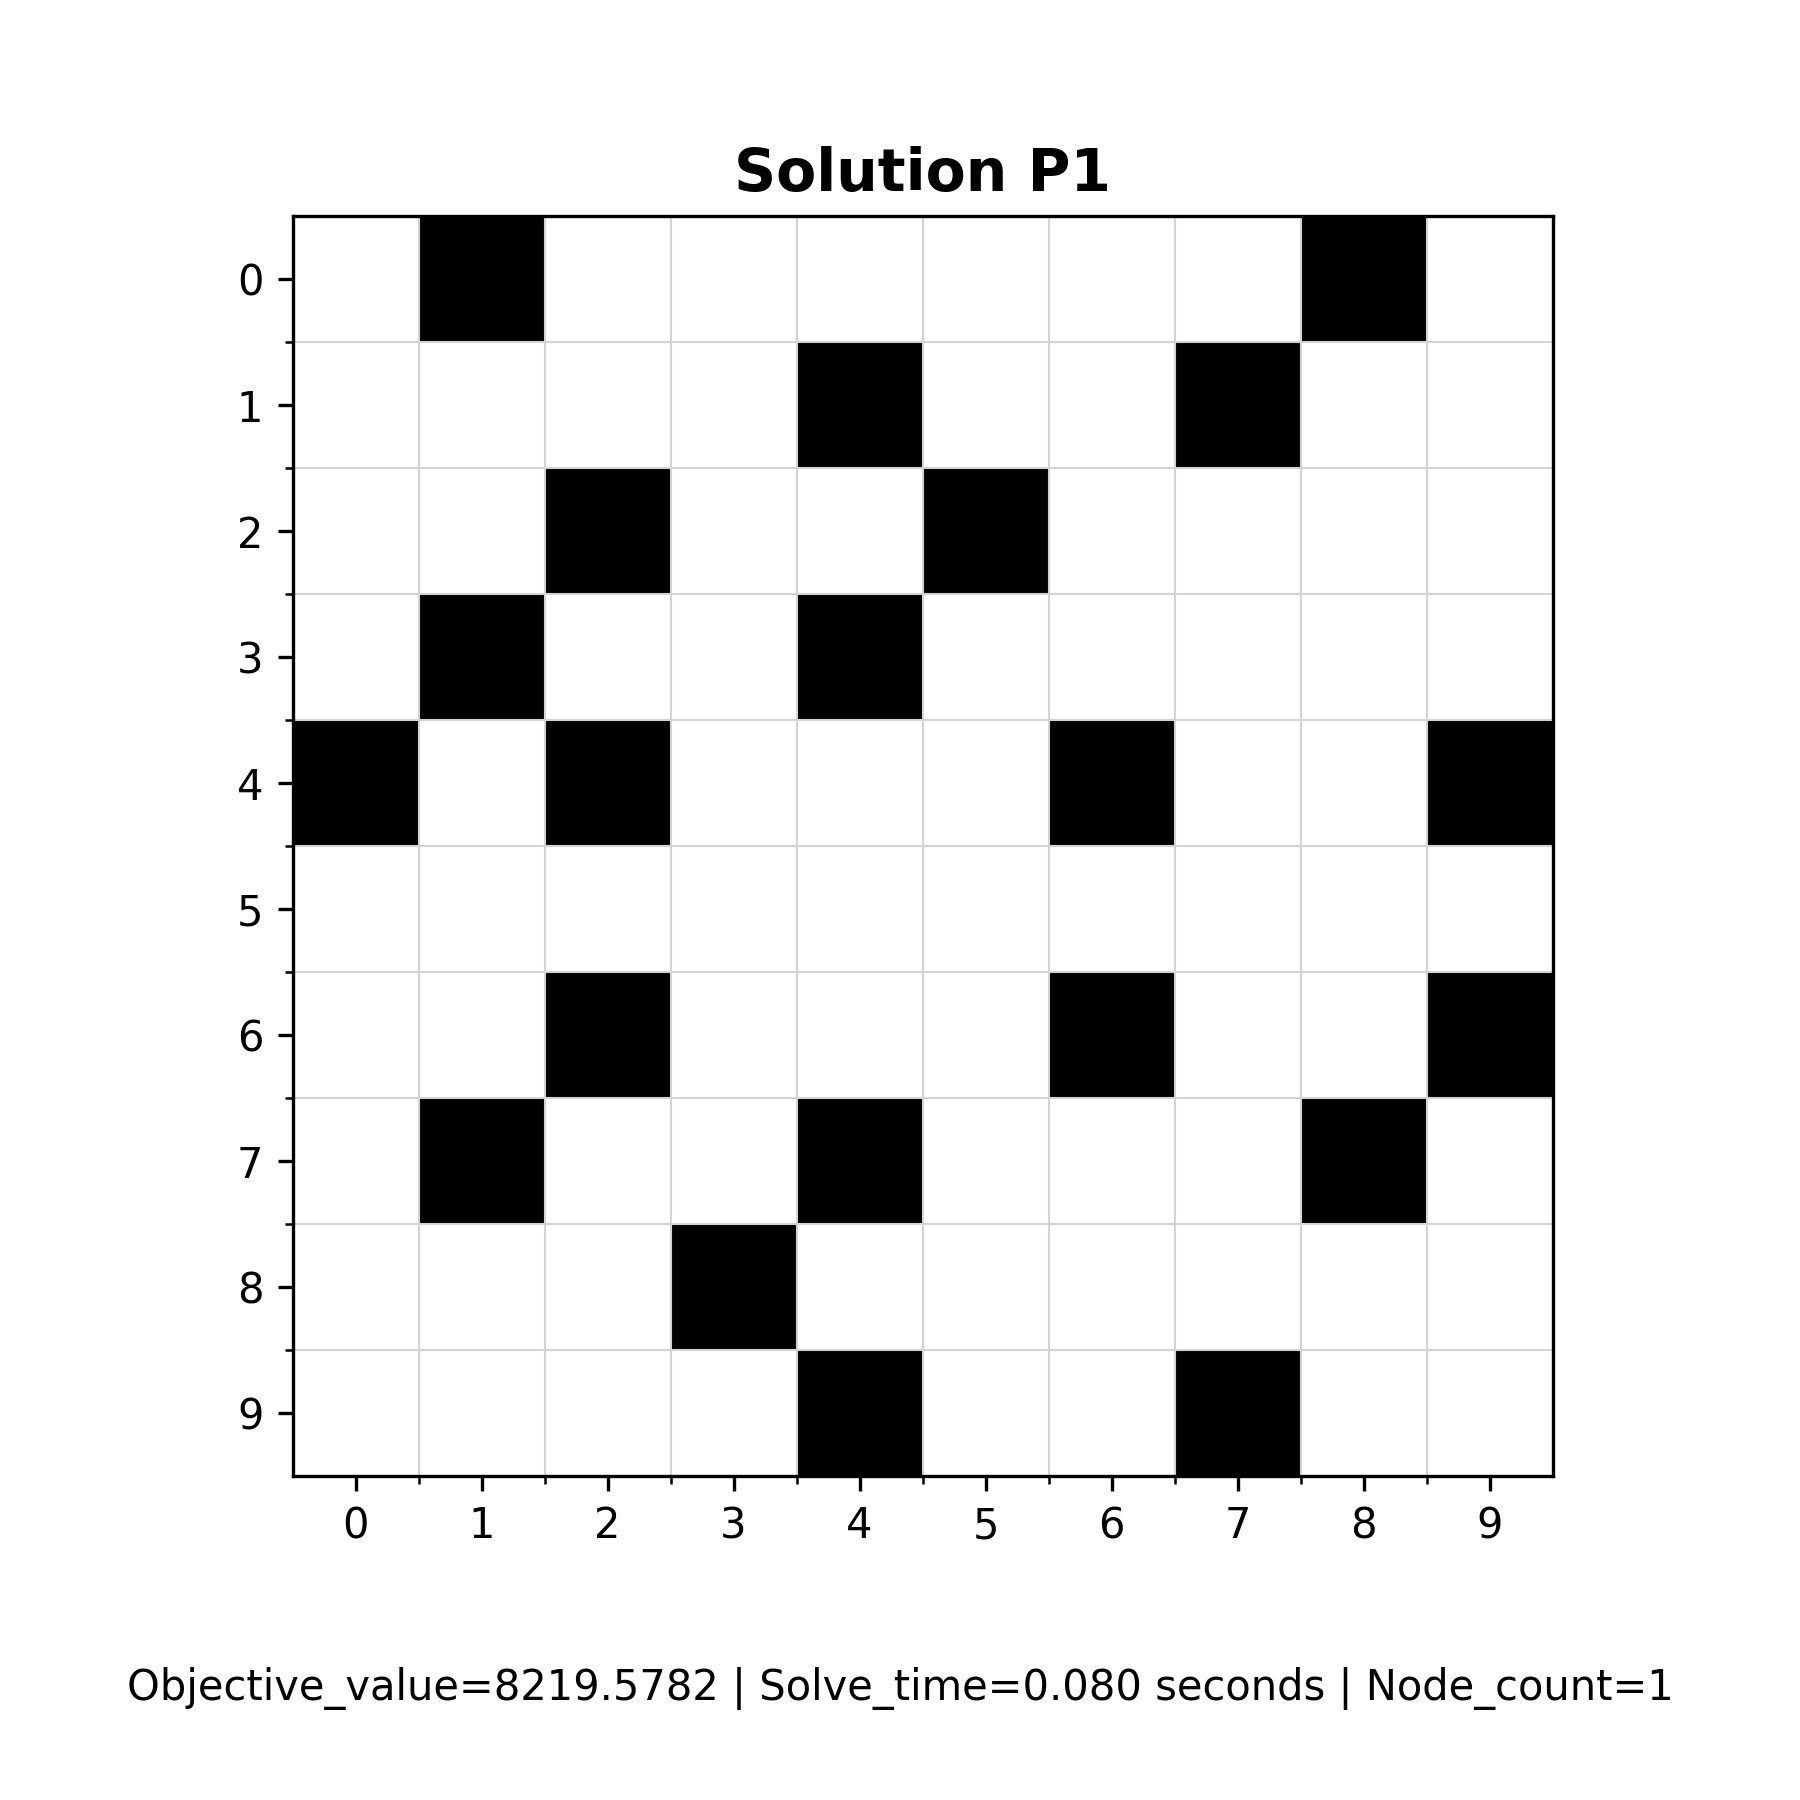
\includegraphics[width=0.7\textwidth]{figs/P1_solution_instance1.png}
\end{figure}
\begin{figure}[H]
  \centering
  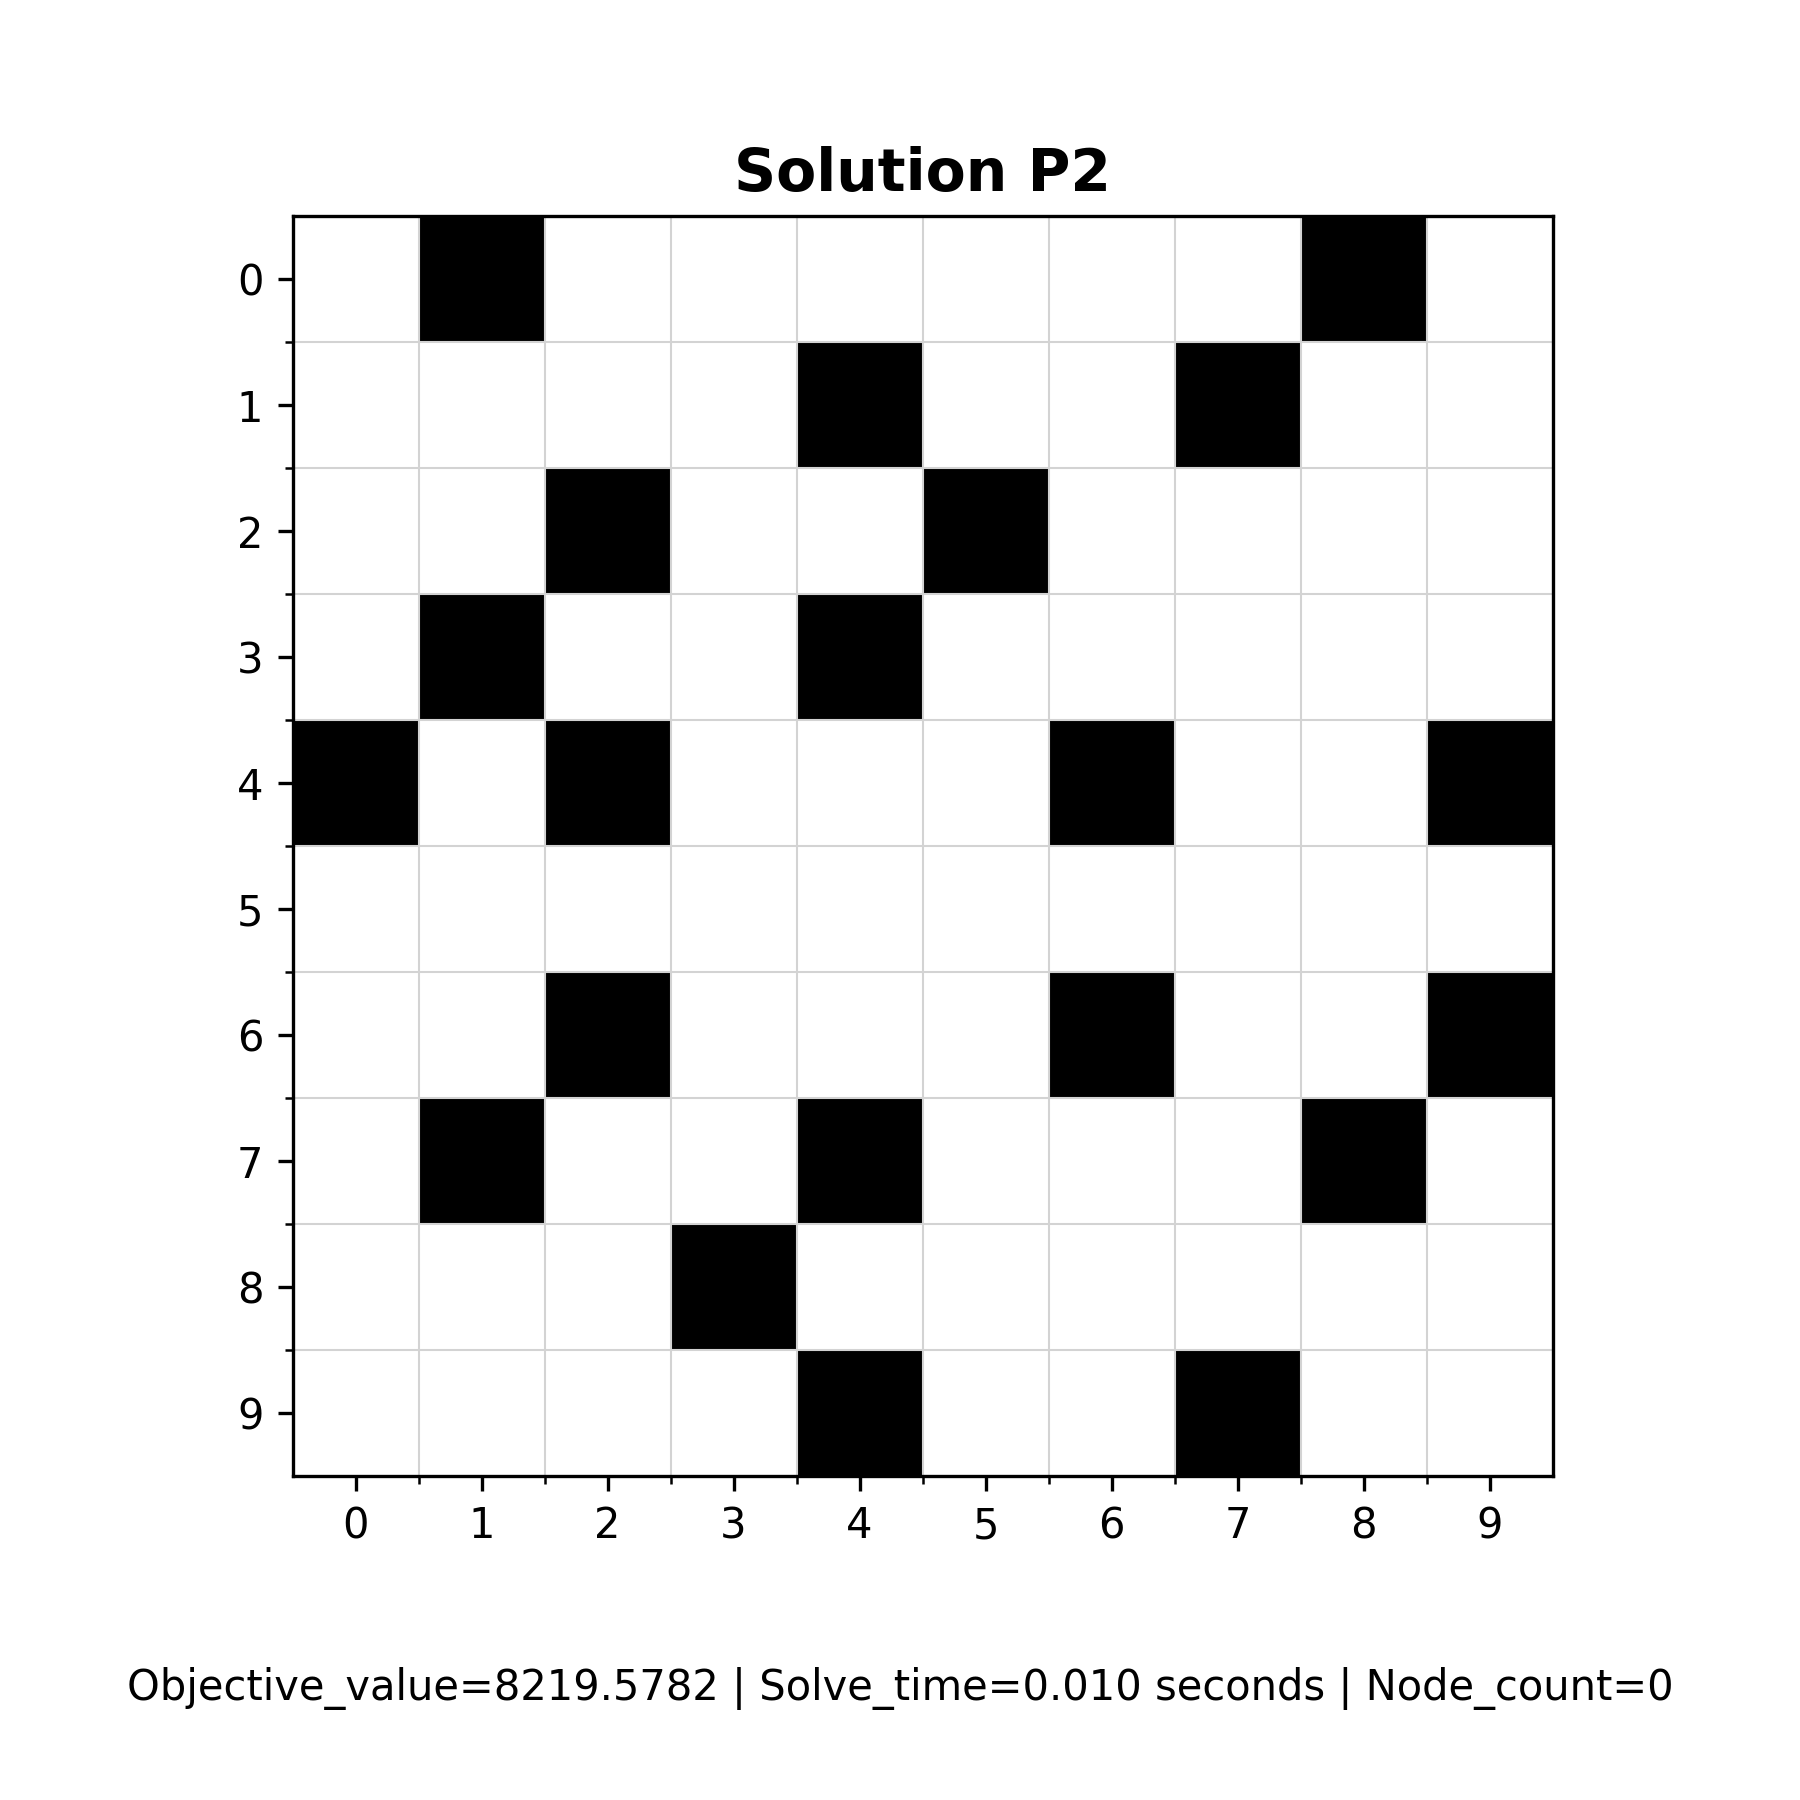
\includegraphics[width=0.7\textwidth]{figs/P2_solution_instance1.png}
\end{figure}
\subsection{Instance 2}
\begin{figure}[H]
  \centering
  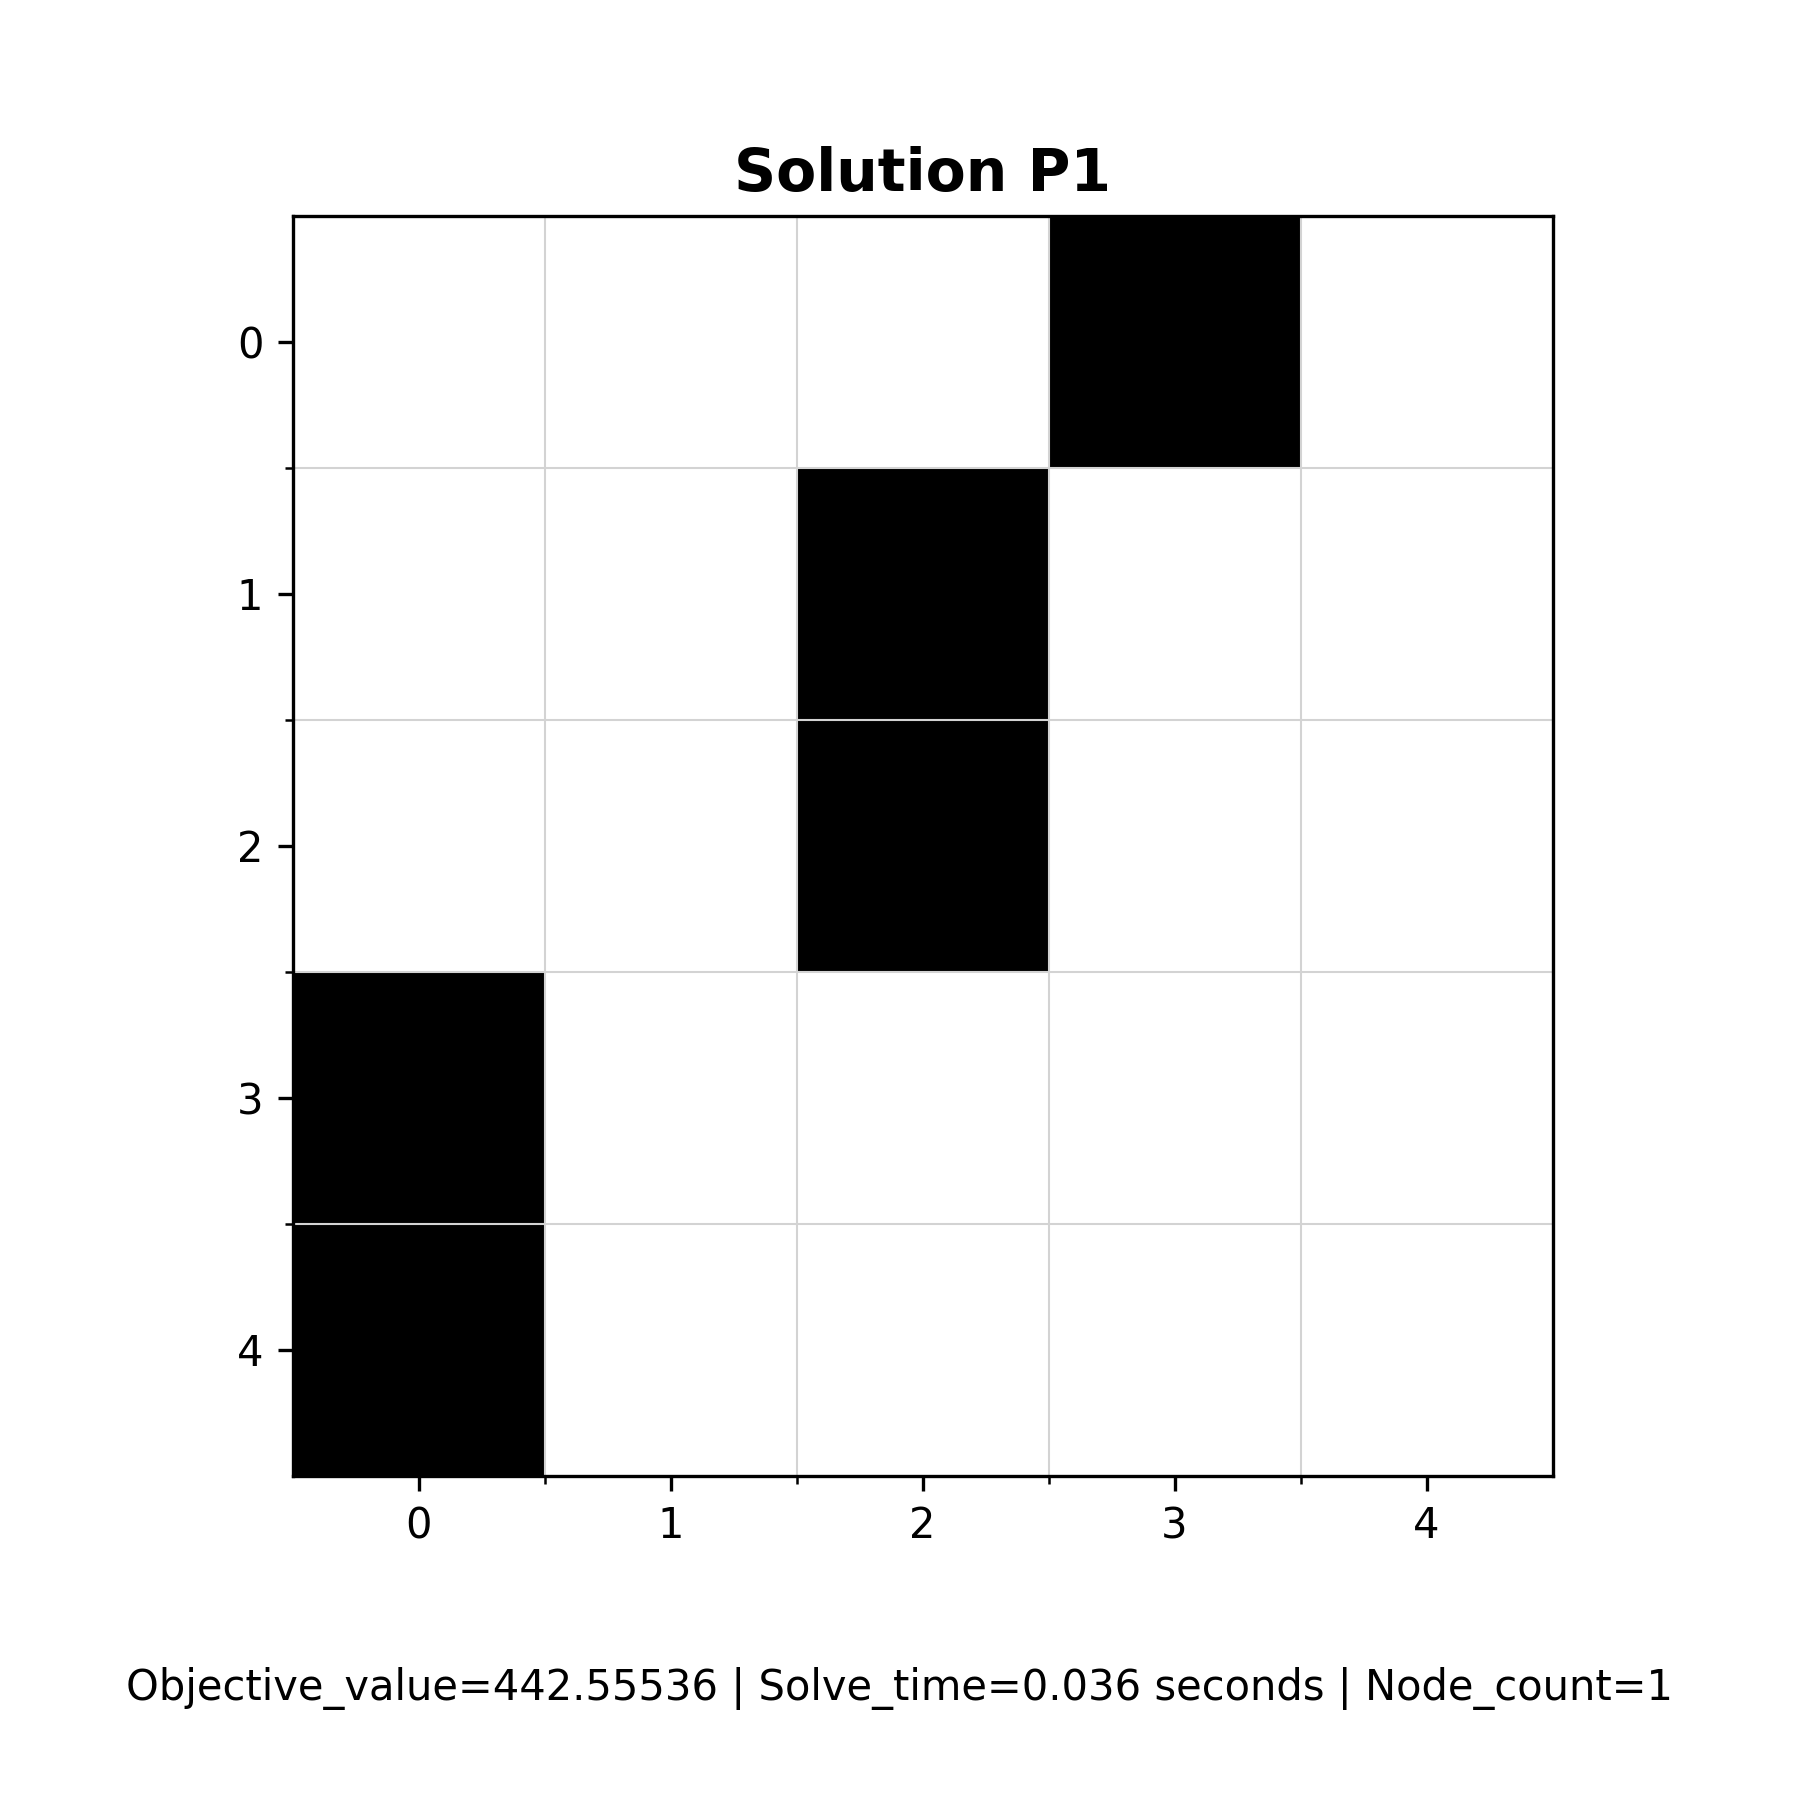
\includegraphics[width=0.7\textwidth]{figs/P1_solution_instance2.png}
\end{figure}
\begin{figure}[H]
  \centering
  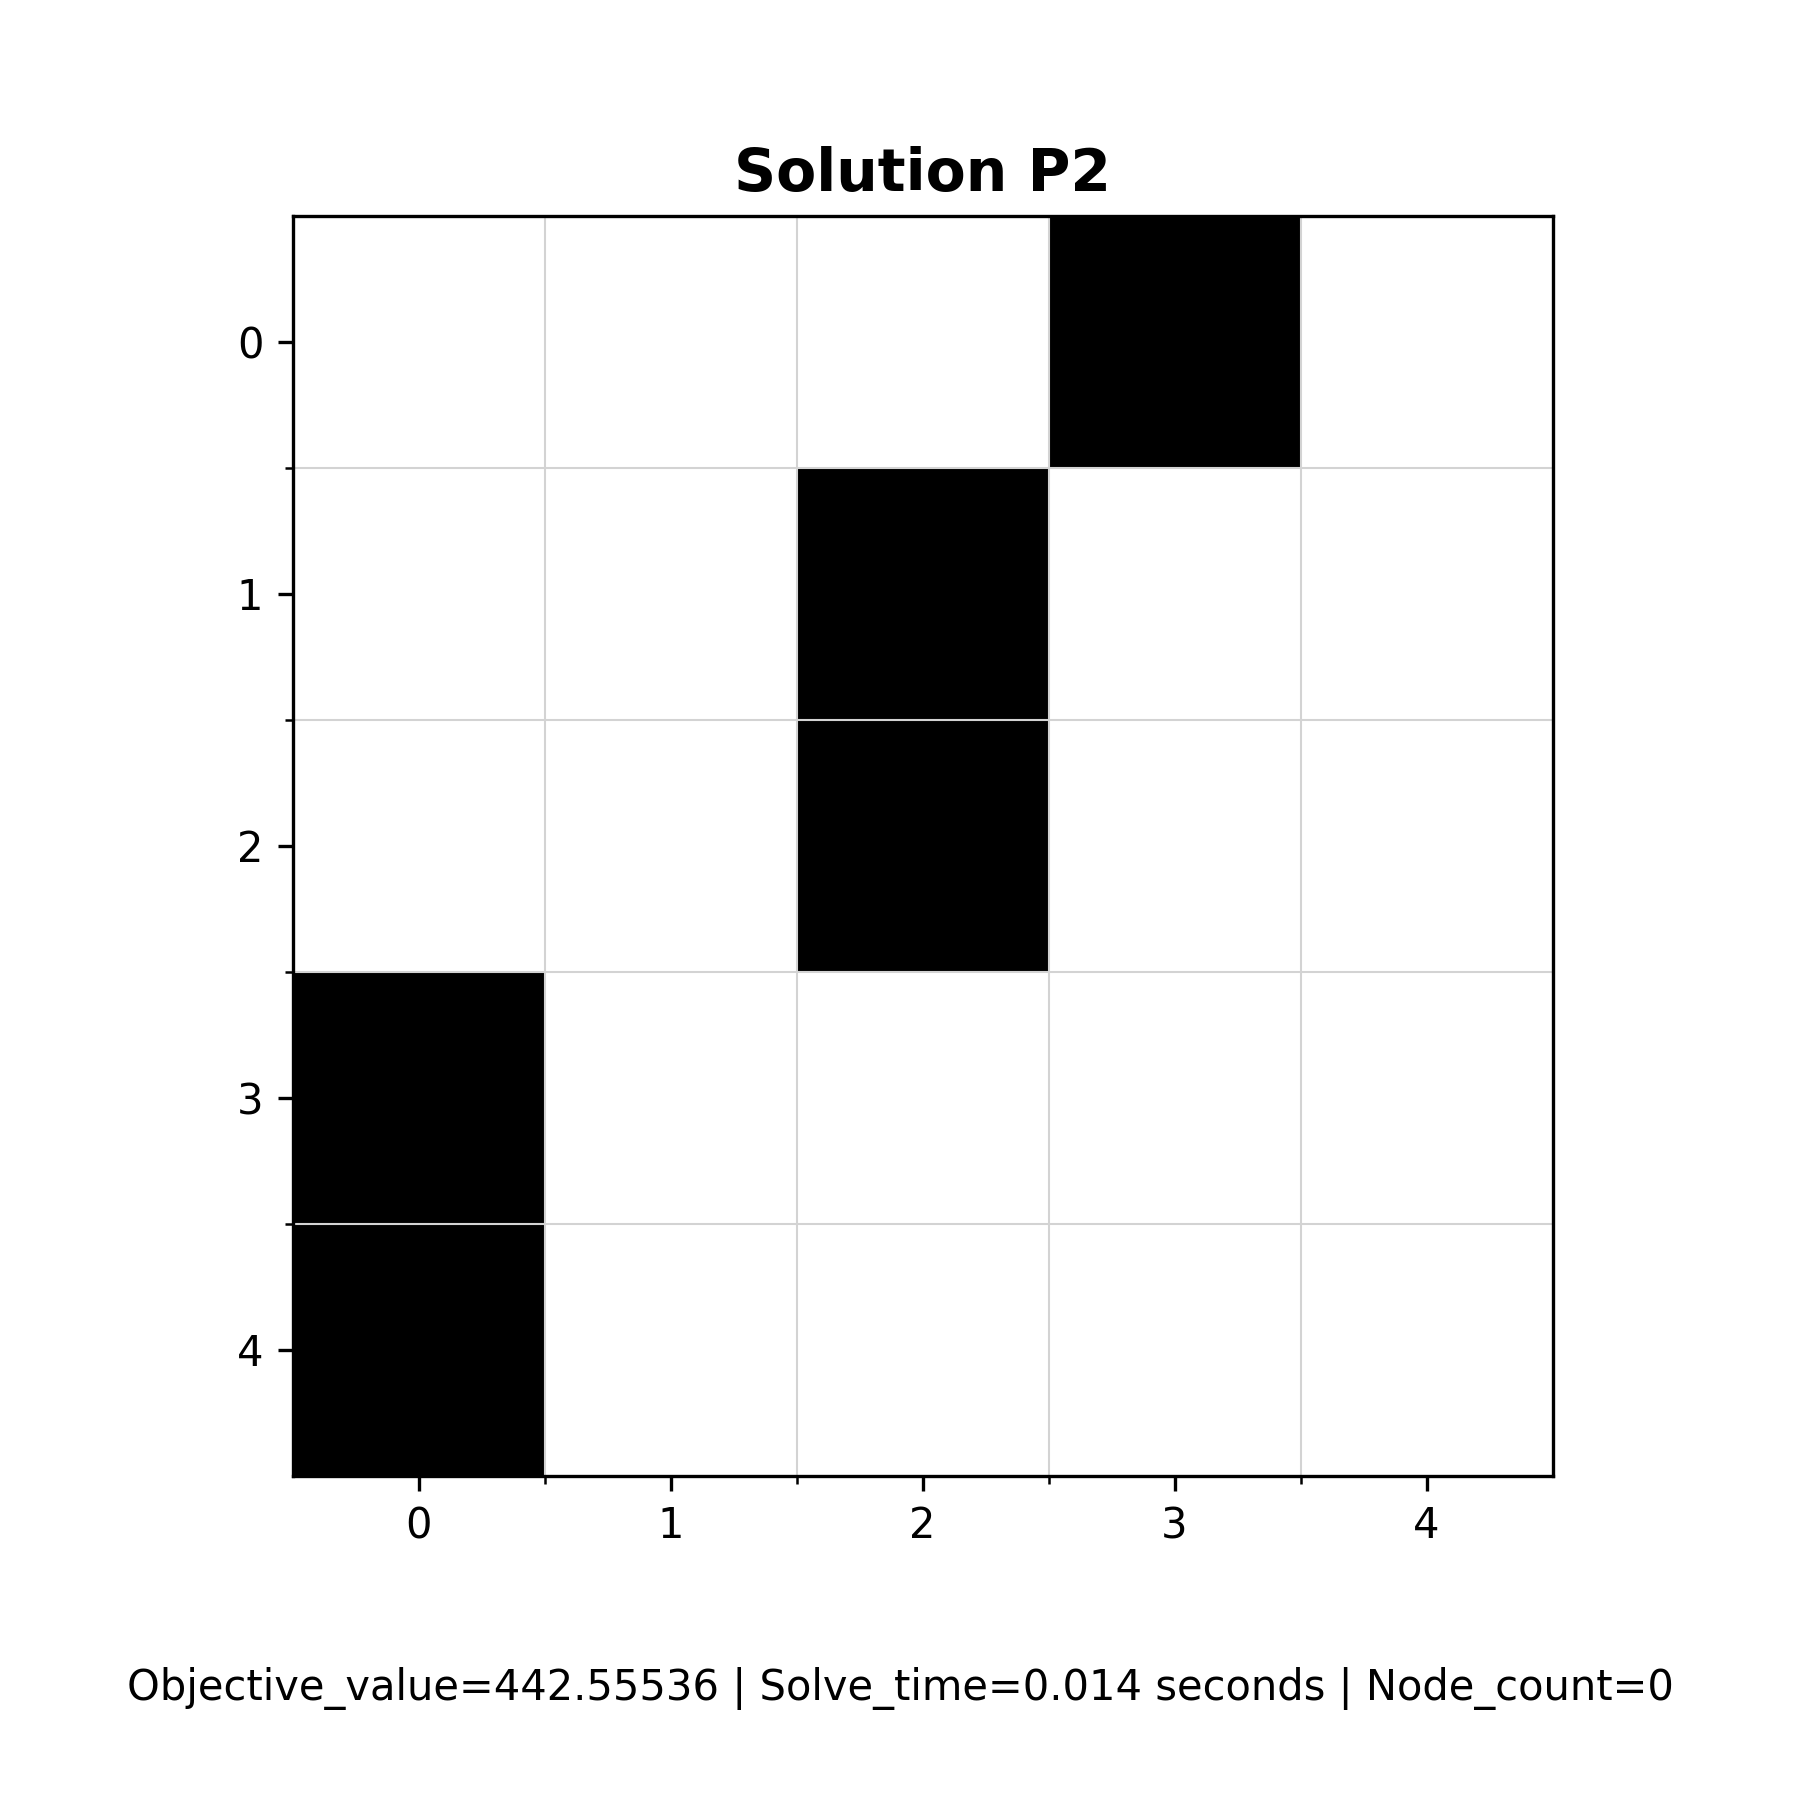
\includegraphics[width=0.7\textwidth]{figs/P2_solution_instance2.png}
\end{figure}

Les solutions sont cohérentes avec le résultat attendu dans l'énoncé (même valeur optimale). 
Il n'y a pas de noeud pour la résolution de P2 car on a directement résolu à l'aide du simplexe. P2 est significativement plus rapide à résoudre que P1. 
C'est cohérent compte tenu que les problèmes de la Programmation linéaire Continue (problème P) et de la Programmation linéaire en variable mixte 
(problème NP-difficile) ne sont pas dans les mêmes classes de complexité (si P != NP)
\subsection{Ajout de la contrainte sur le nombre de parcelles non coupées}

On ajoute maintenant la contrainte de cardinalité imposant que le nombre de parcelles non coupées soit supérieur ou égal à une borne $B$ :
\[
\sum_{(i,j)}  x_{ij} \ge B
\]
ce qui revient à ajouter une ligne dont tous les coefficients associés aux variables $x_{ij}$ valent $1$, et des zéros sur les colonnes associées aux variables $y_{ijkl}$.
La nouvelle matrice des contraintes devient donc :
\[
\begin{bmatrix}
A & -I \\
I   & 0 \\
0   & I \\
1 & 0
\end{bmatrix}
\]

\vspace{0.5cm}
\noindent
\textbf{Perte de la TU : contre-exemple pour $m=n=3$.}

\noindent
Pour montrer que la matrice des contraintes n’est plus totalement unimodulaire, il suffit d’exhiber une sous-matrice carrée de déterminant de module strictement supérieur à 1.

On considère les colonnes correspondant aux variables $x_{02}$, $x_{11}$, $x_{12}$ et $x_{22}$, et les lignes associées :
\begin{itemize}
    \item aux contraintes de type (i) contenant respectivement les variables 
    $y_{(1,2)(0,2)}$, $y_{(1,2)(1,1)}$, $y_{(1,2)(2,2)}$ ;
    \item ainsi qu’à la contrainte de cardinalité nouvellement ajoutée.
\end{itemize}

La sous-matrice extraite est donc :
\[
M =
\begin{pmatrix}
1 & 0 & 1 & 0 \\[3pt]
0 & 1 & 1 & 0 \\[3pt]
0 & 0 & 1 & 1 \\[3pt]
1 & 1 & 1 & 1
\end{pmatrix}.
\]

On calcule alors son déterminant :
\[
\det(M)
= 
\begin{vmatrix}
1 & 0 & 1 & 0 \\
0 & 1 & 1 & 0 \\
0 & 0 & 1 & 1 \\
1 & 1 & 1 & 1
\end{vmatrix}.
\]
En effectuant les opérations élémentaires sur les lignes 
$\text{L}_4 \leftarrow \text{L}_4 - (\text{L}_1 + \text{L}_2 + \text{L}_3)$,
on obtient :
\[
\begin{pmatrix}
1 & 0 & 1 & 0 \\
0 & 1 & 1 & 0 \\
0 & 0 & 1 & 1 \\
0 & 0 & -2 & 0
\end{pmatrix},
\]
dont le déterminant vaut en développant sur la dernière ligne (on fait apparaitre une matrice identité 3x3)
\[
\det(M) = (-1)^{4+3} \times -2 \times det(I_3)= 2.
\]

\vspace{0.3cm}
\noindent
Ainsi, $\det(M) = 2 \notin \{-1,0,1\}$, ce qui prouve que la matrice des contraintes n’est pas totalement unimodulaire.
L’ajout de la contrainte sur le nombre minimal de parcelles non coupées fait donc, en général, perdre la propriété de totale unimodularité du système.
Donc on ne peut pas à priori pas résoudre avec l'algorithme du simplexe le problème avec des contraintes sur le nombre de parcelles non coupées.
\subsection{Résolutions des instances}
On résout l'instance 10x10 en ajoutant la contrainte sur le nombre de parcelles non coupées. Pour P2 on est obligé de repasser à un modèle de PL-01. 
On obtient les résultats suivants :
\begin{figure}[H]
  \centering
  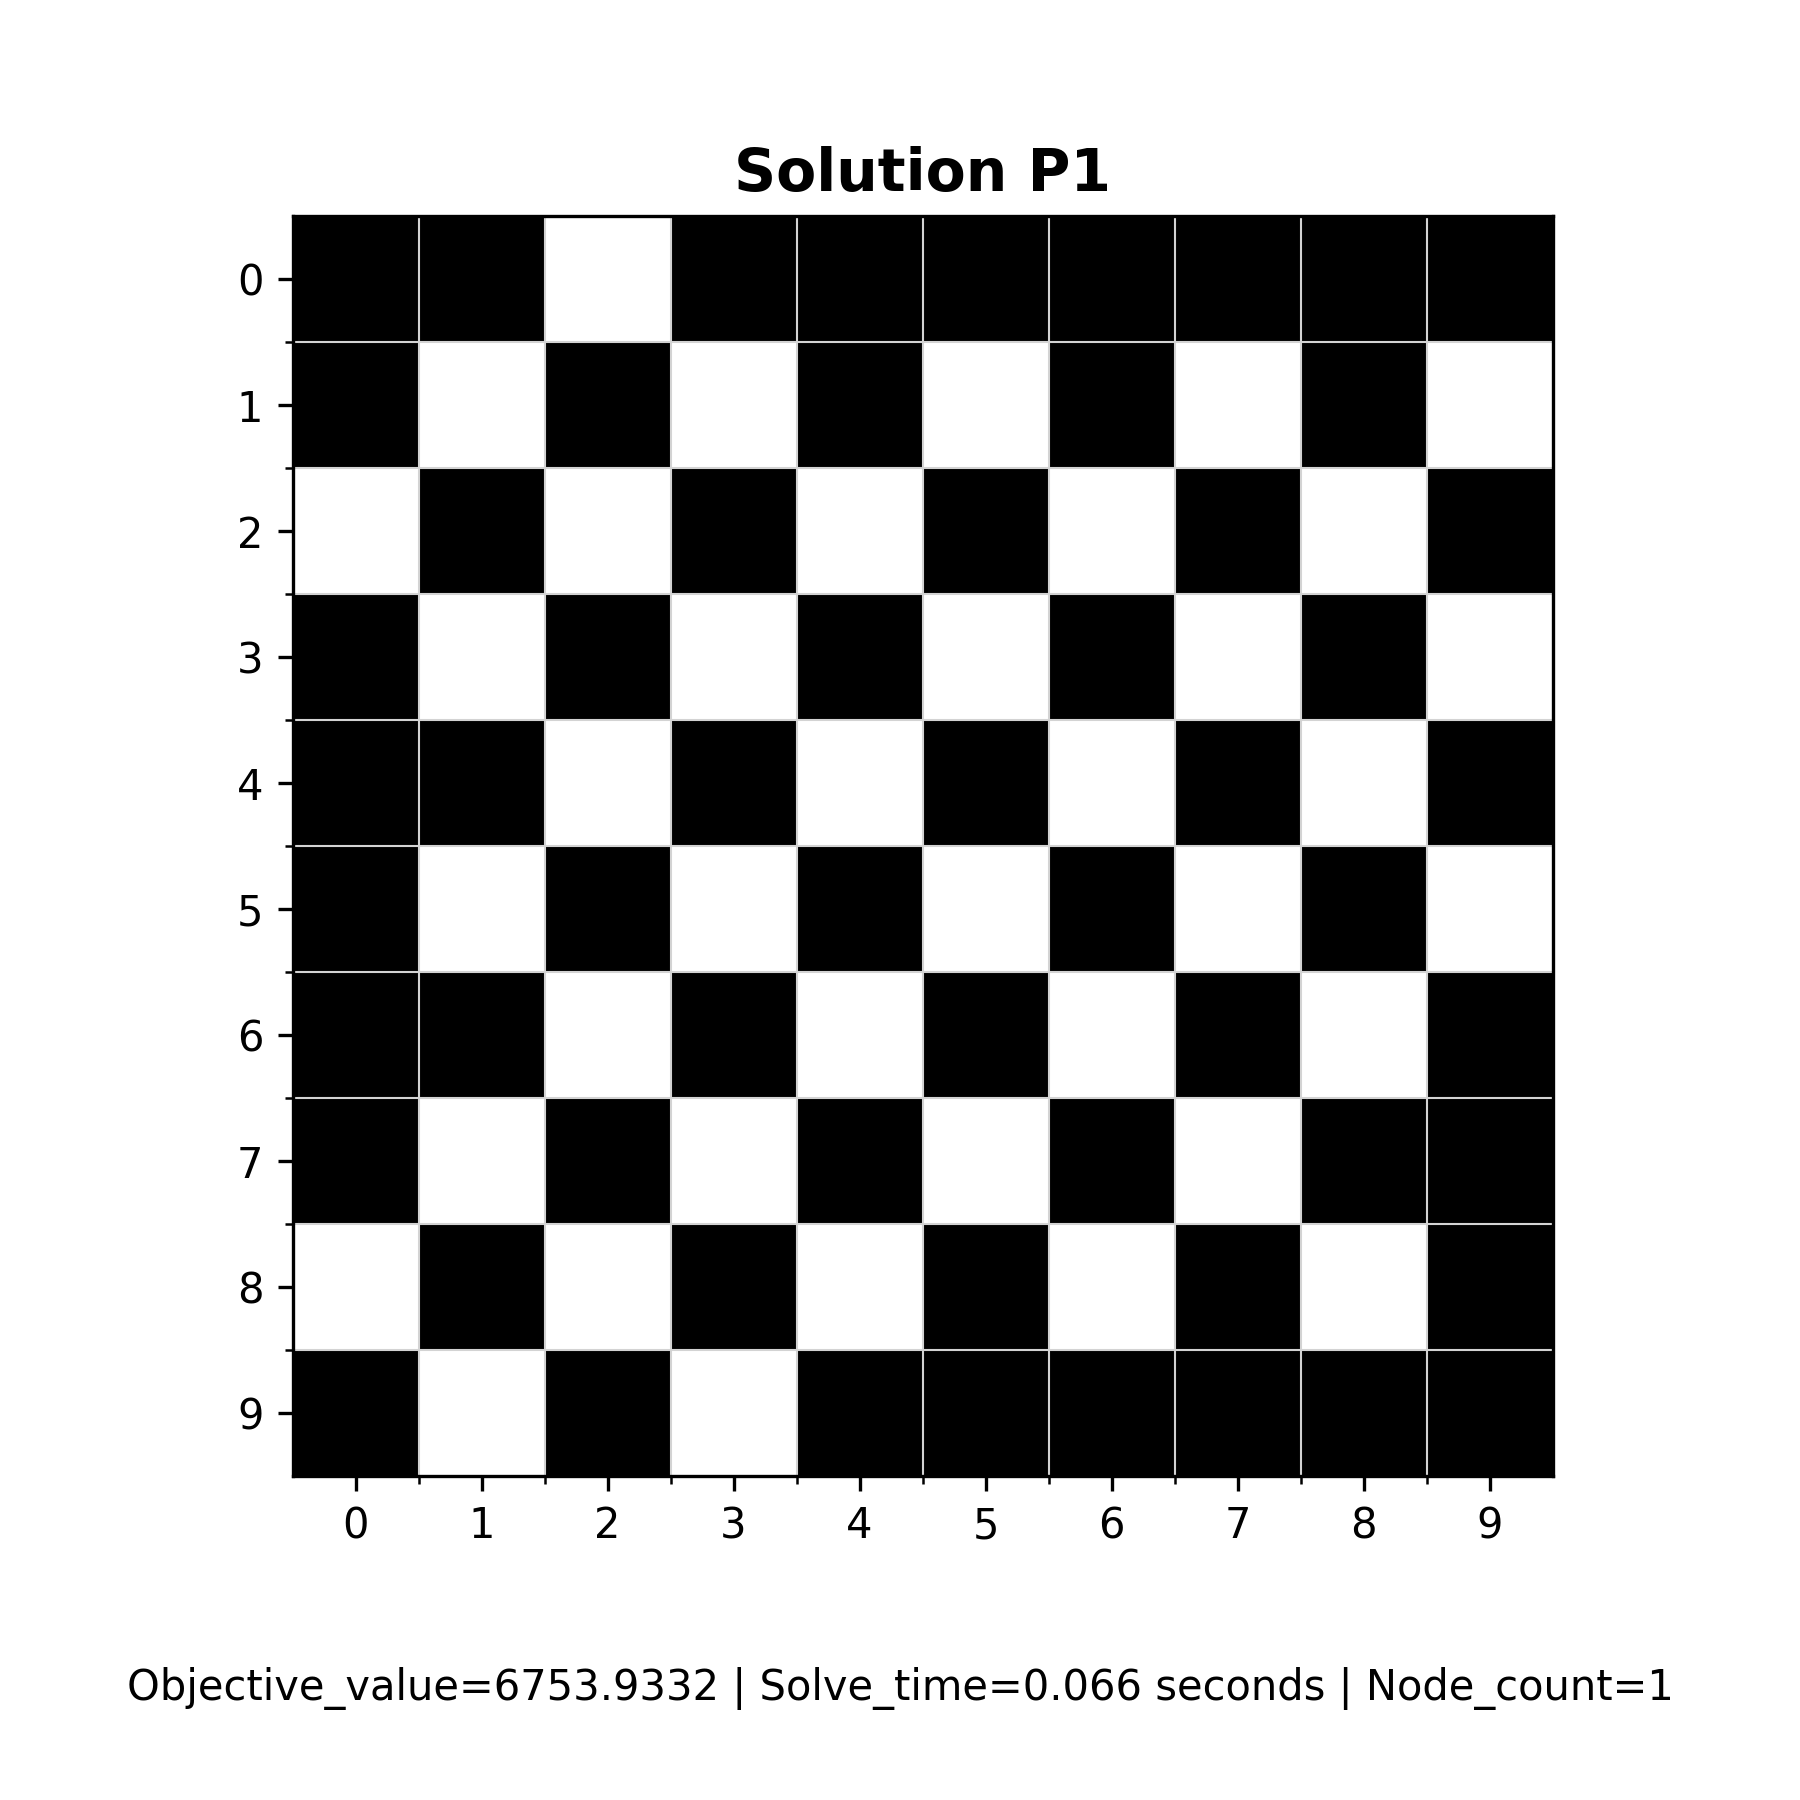
\includegraphics[width=0.7\textwidth]{figs/P1_solution_instance1_B.png}
\end{figure}
\begin{figure}[H]
  \centering
  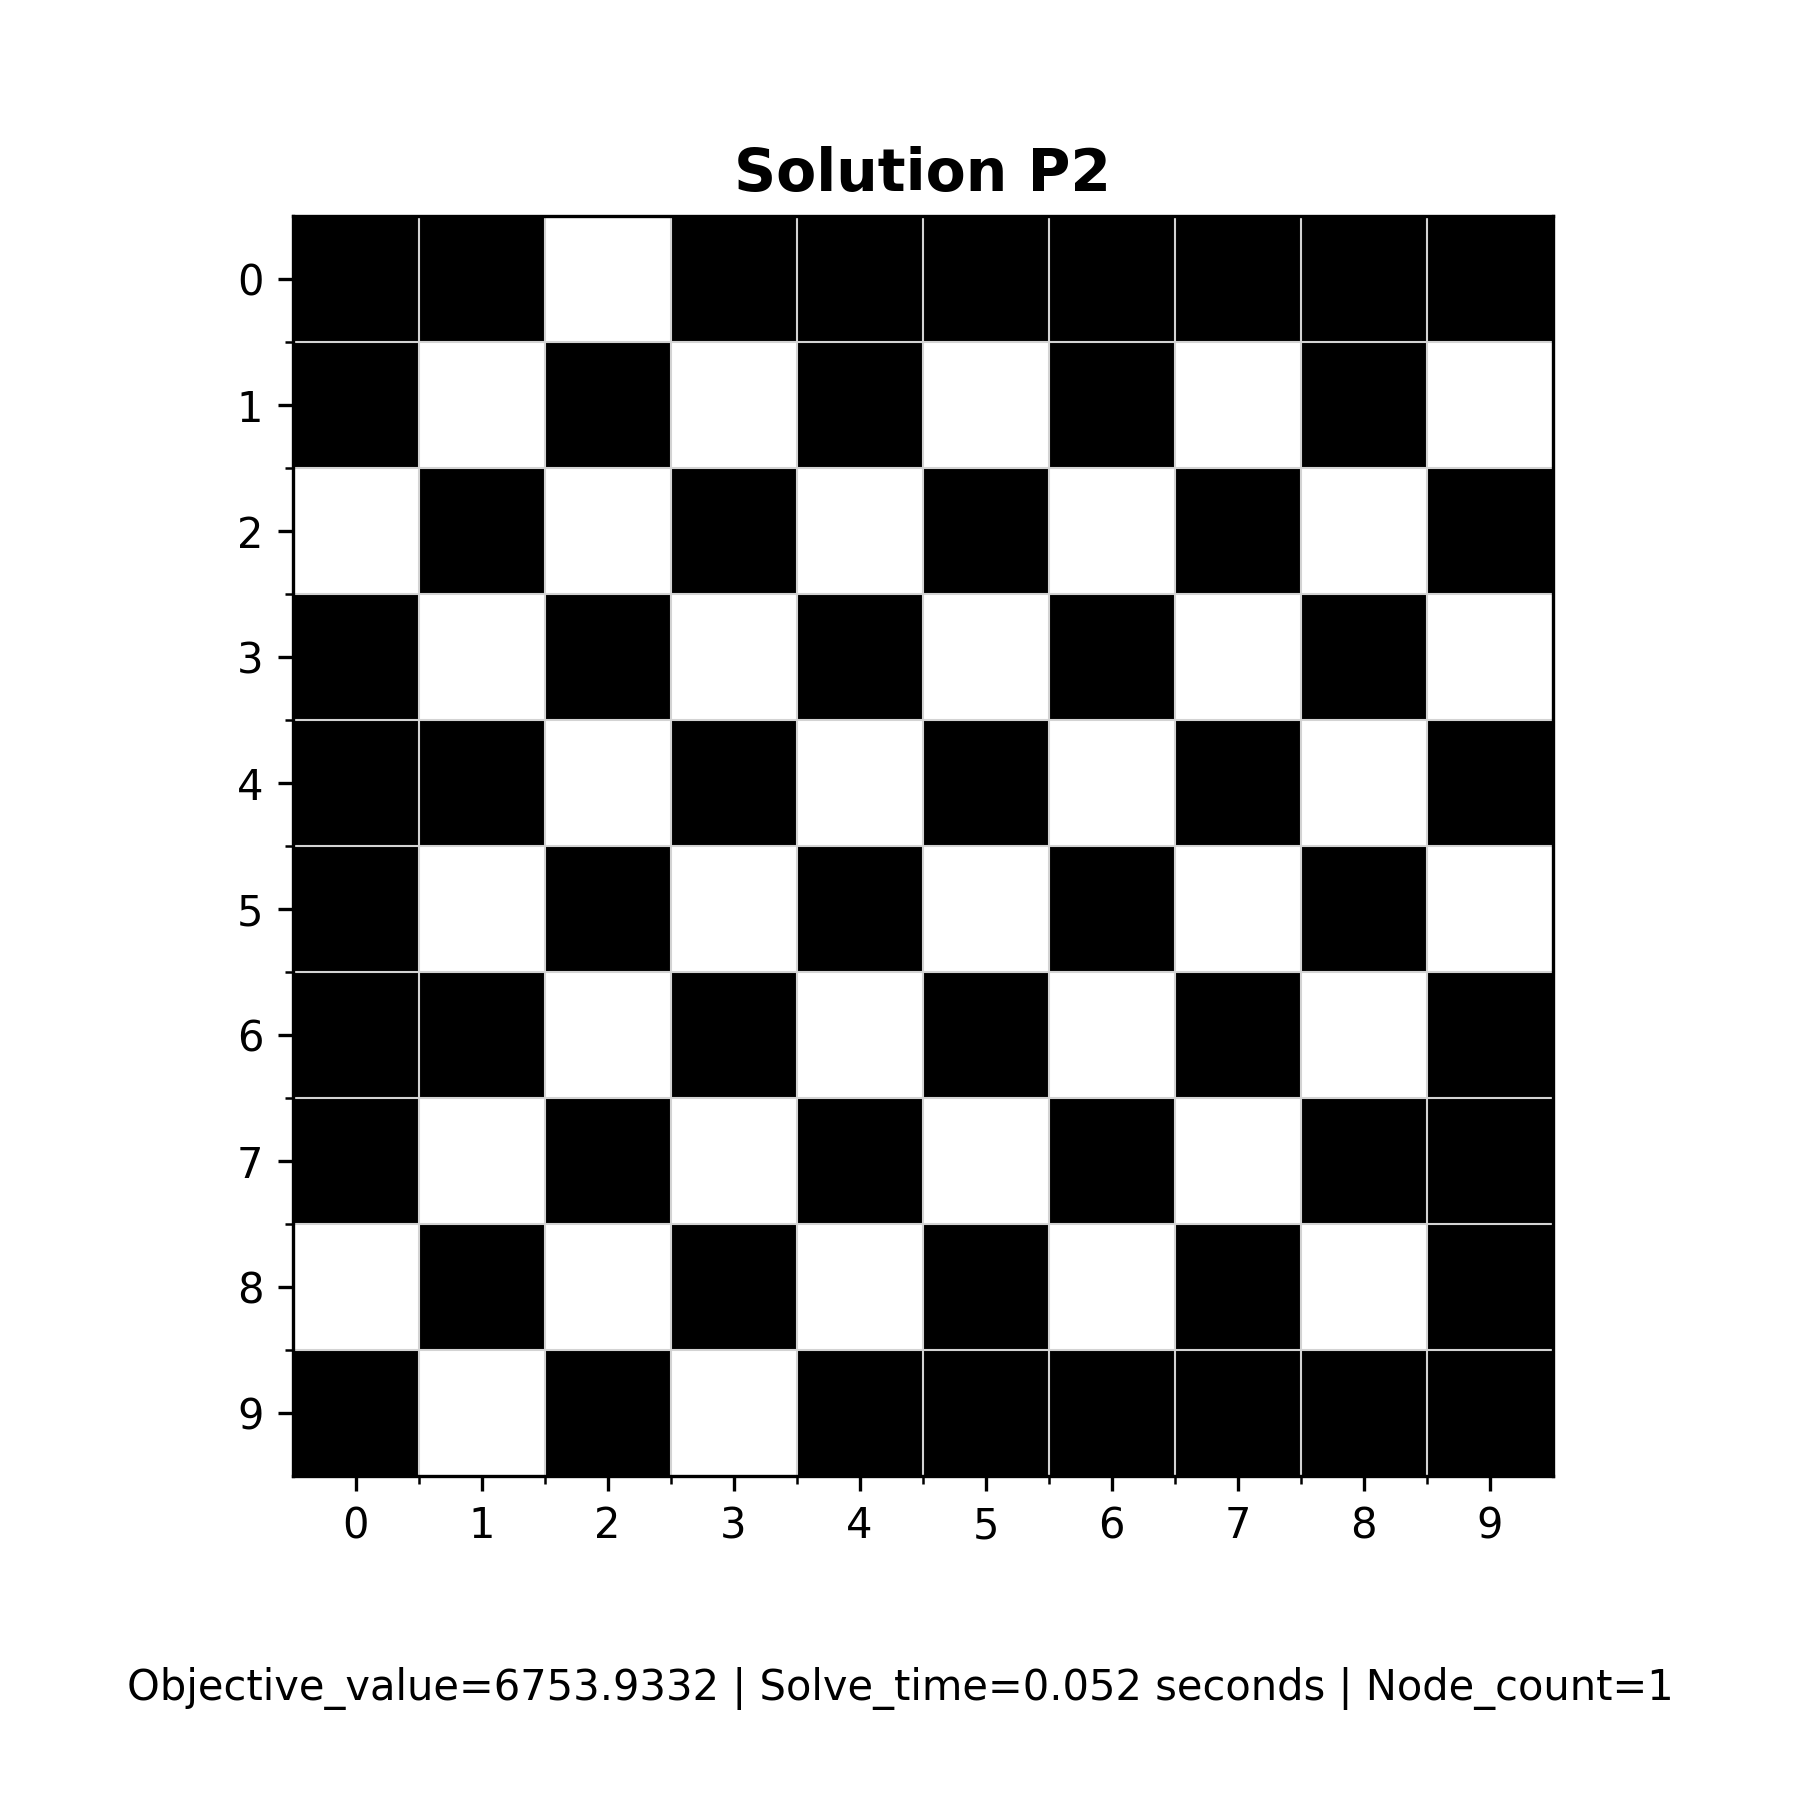
\includegraphics[width=0.7\textwidth]{figs/P2_solution_instance1_B.png}
\end{figure}
\subsection{Comparaison des approches}
On compare les solutions sur des grilles de taille 10 x 10 à 250 x 250. On compare 
la différence de temps de résolution avec et sans la contrainte sur les parcelles non coupées \\
Modèle P1 : \\
Sans la contrainte sur les parcelles non coupées
\begin{figure}[H]
  \centering
  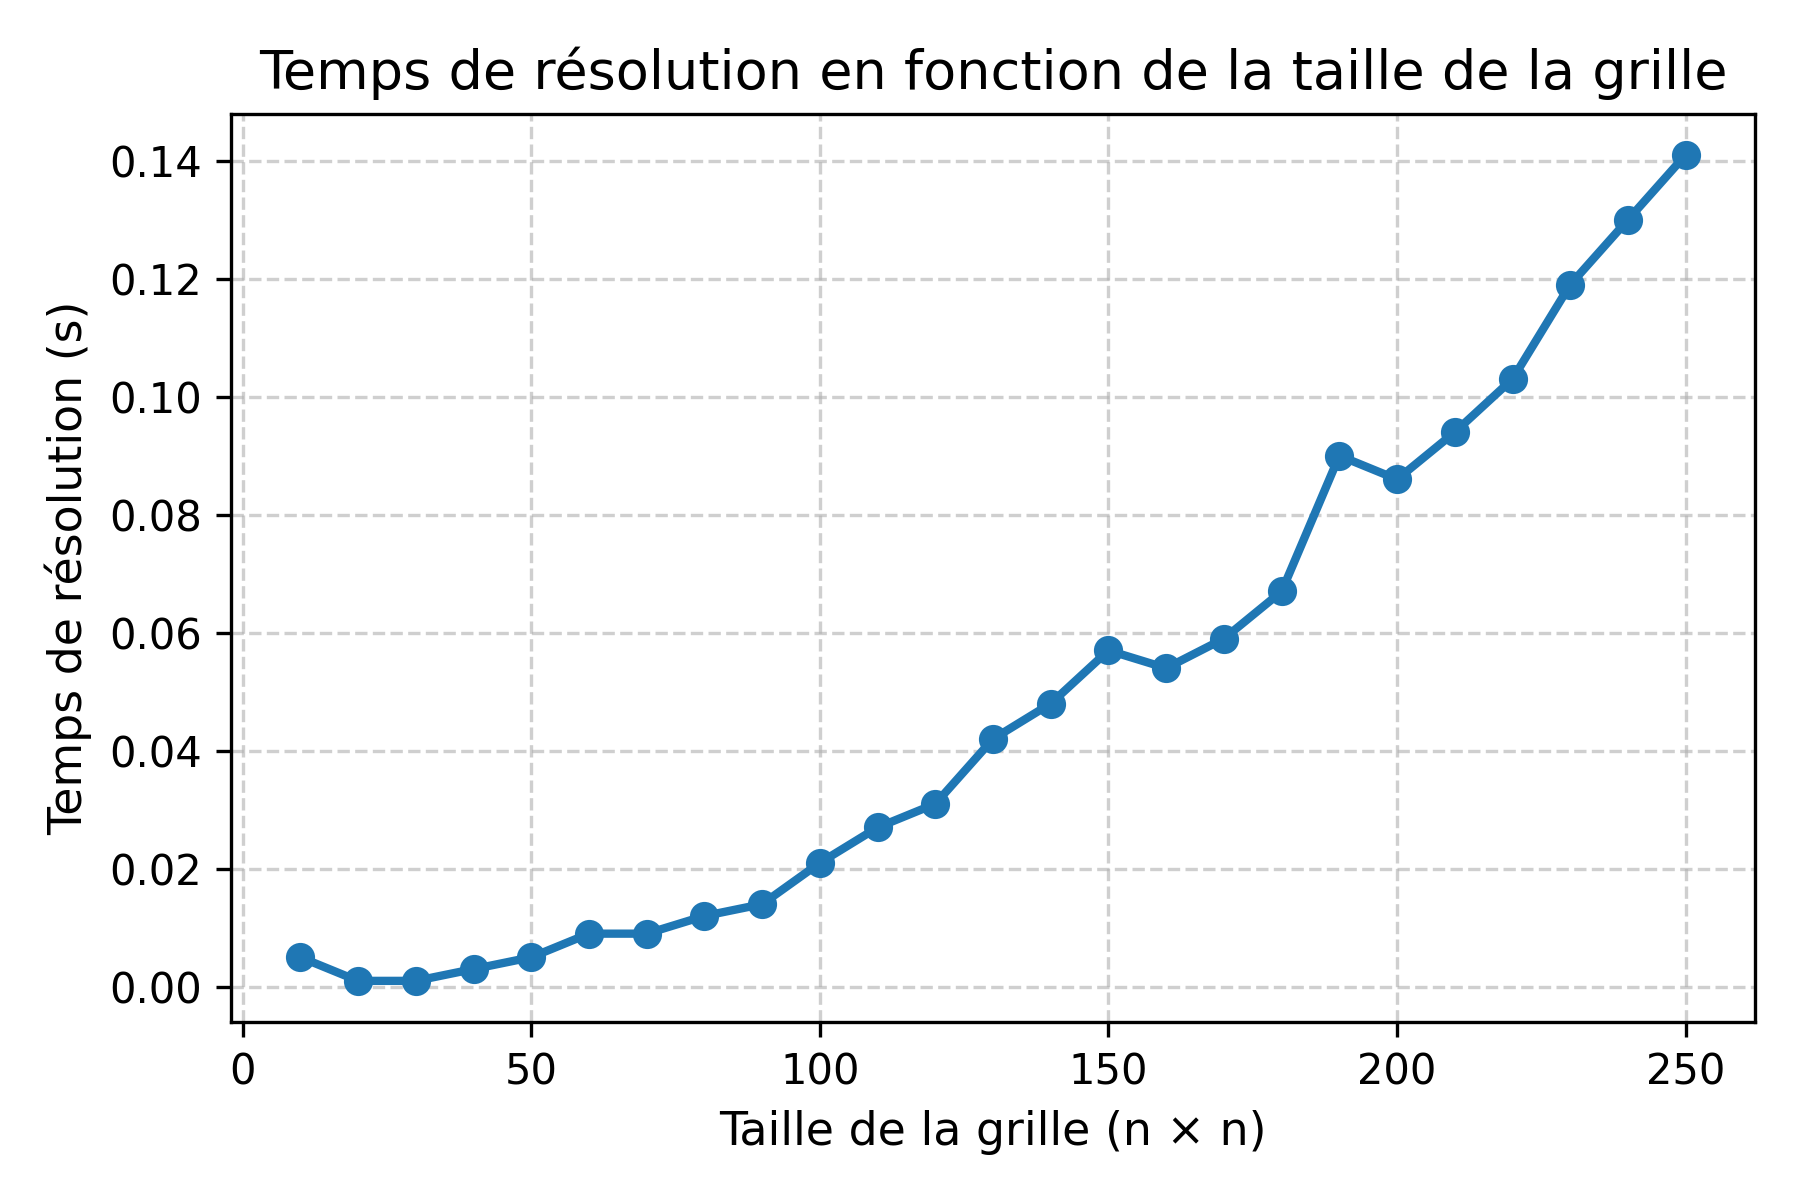
\includegraphics[width=0.7\textwidth]{figs/execution_time_P1_sans_B.png}
\end{figure}
Avec :
\begin{figure}[H]
  \centering
  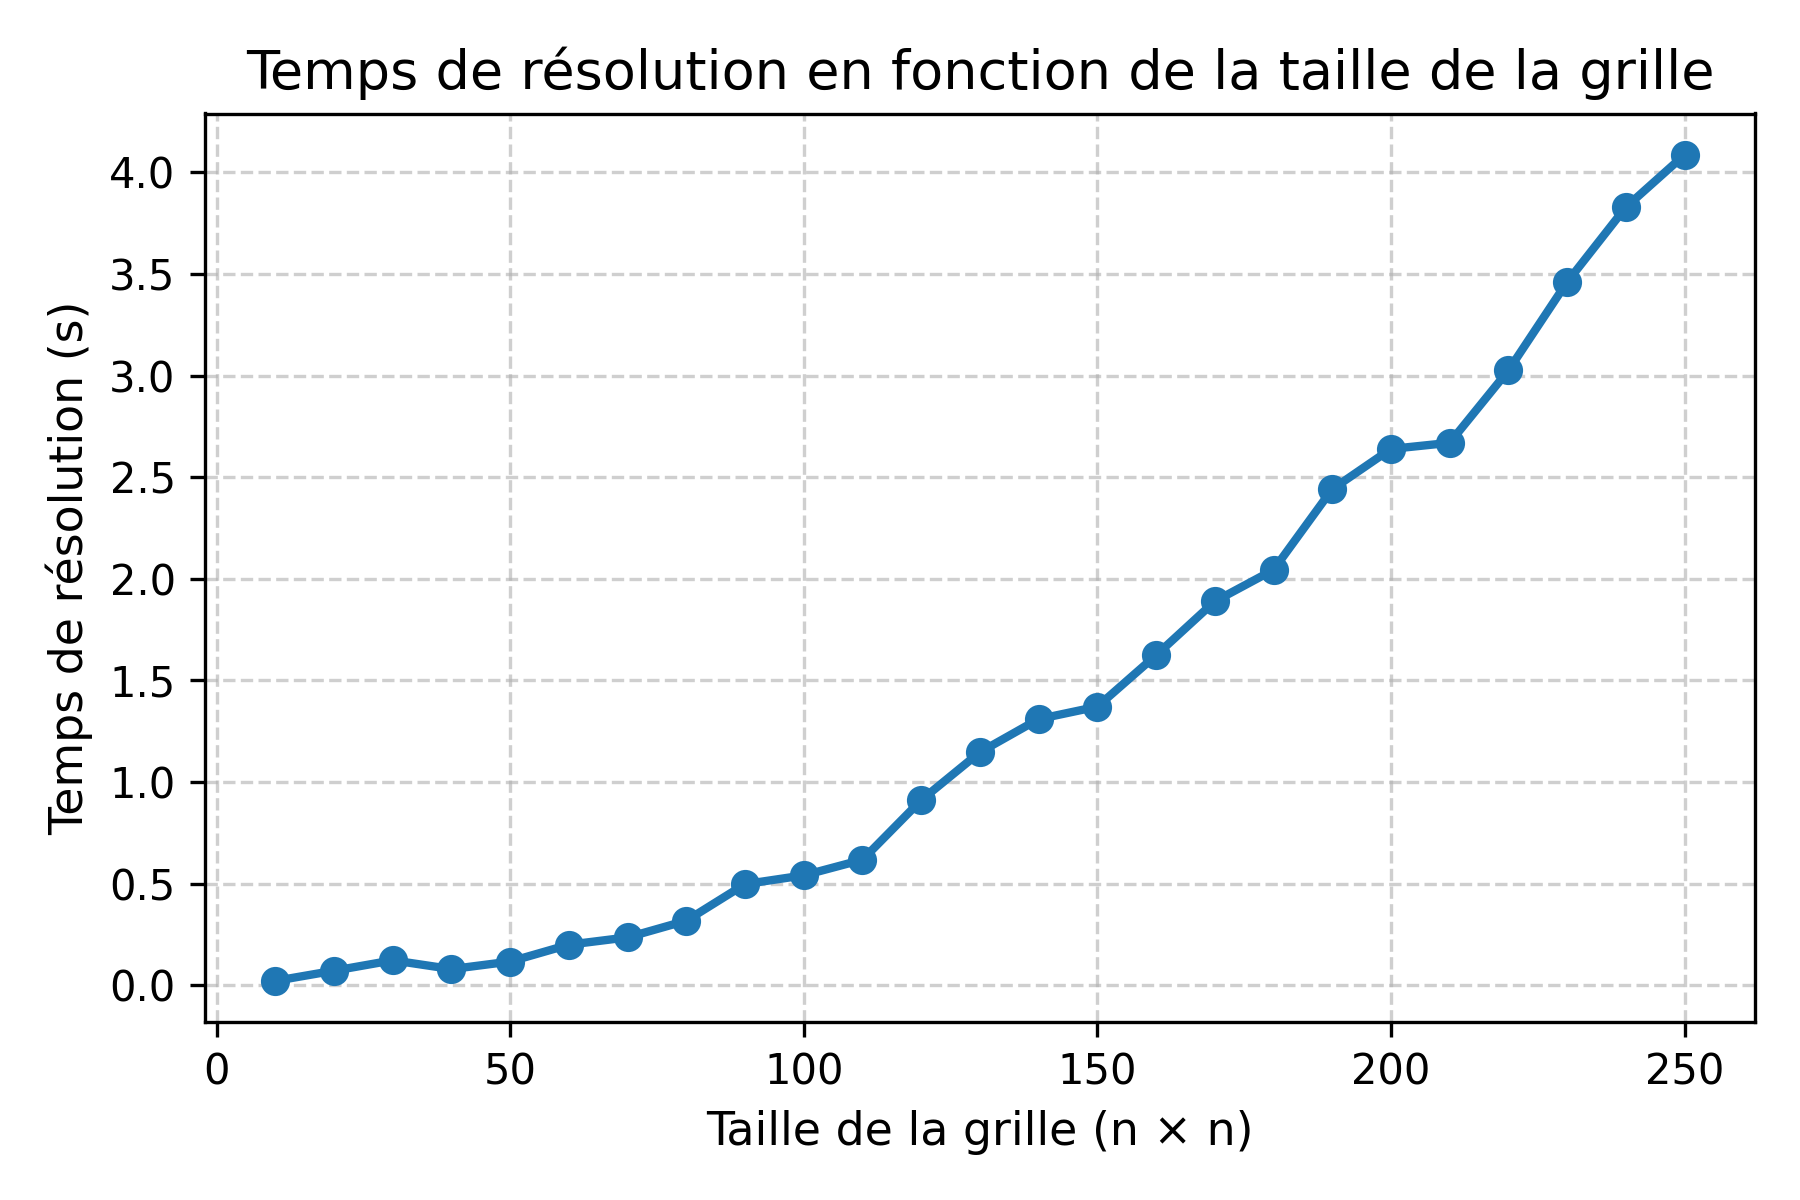
\includegraphics[width=0.7\textwidth]{figs/execution_time_P1_avec_B.png}
\end{figure}
Modèle P2:\\
Avec relaxation continue :
\begin{figure}[H]
  \centering
  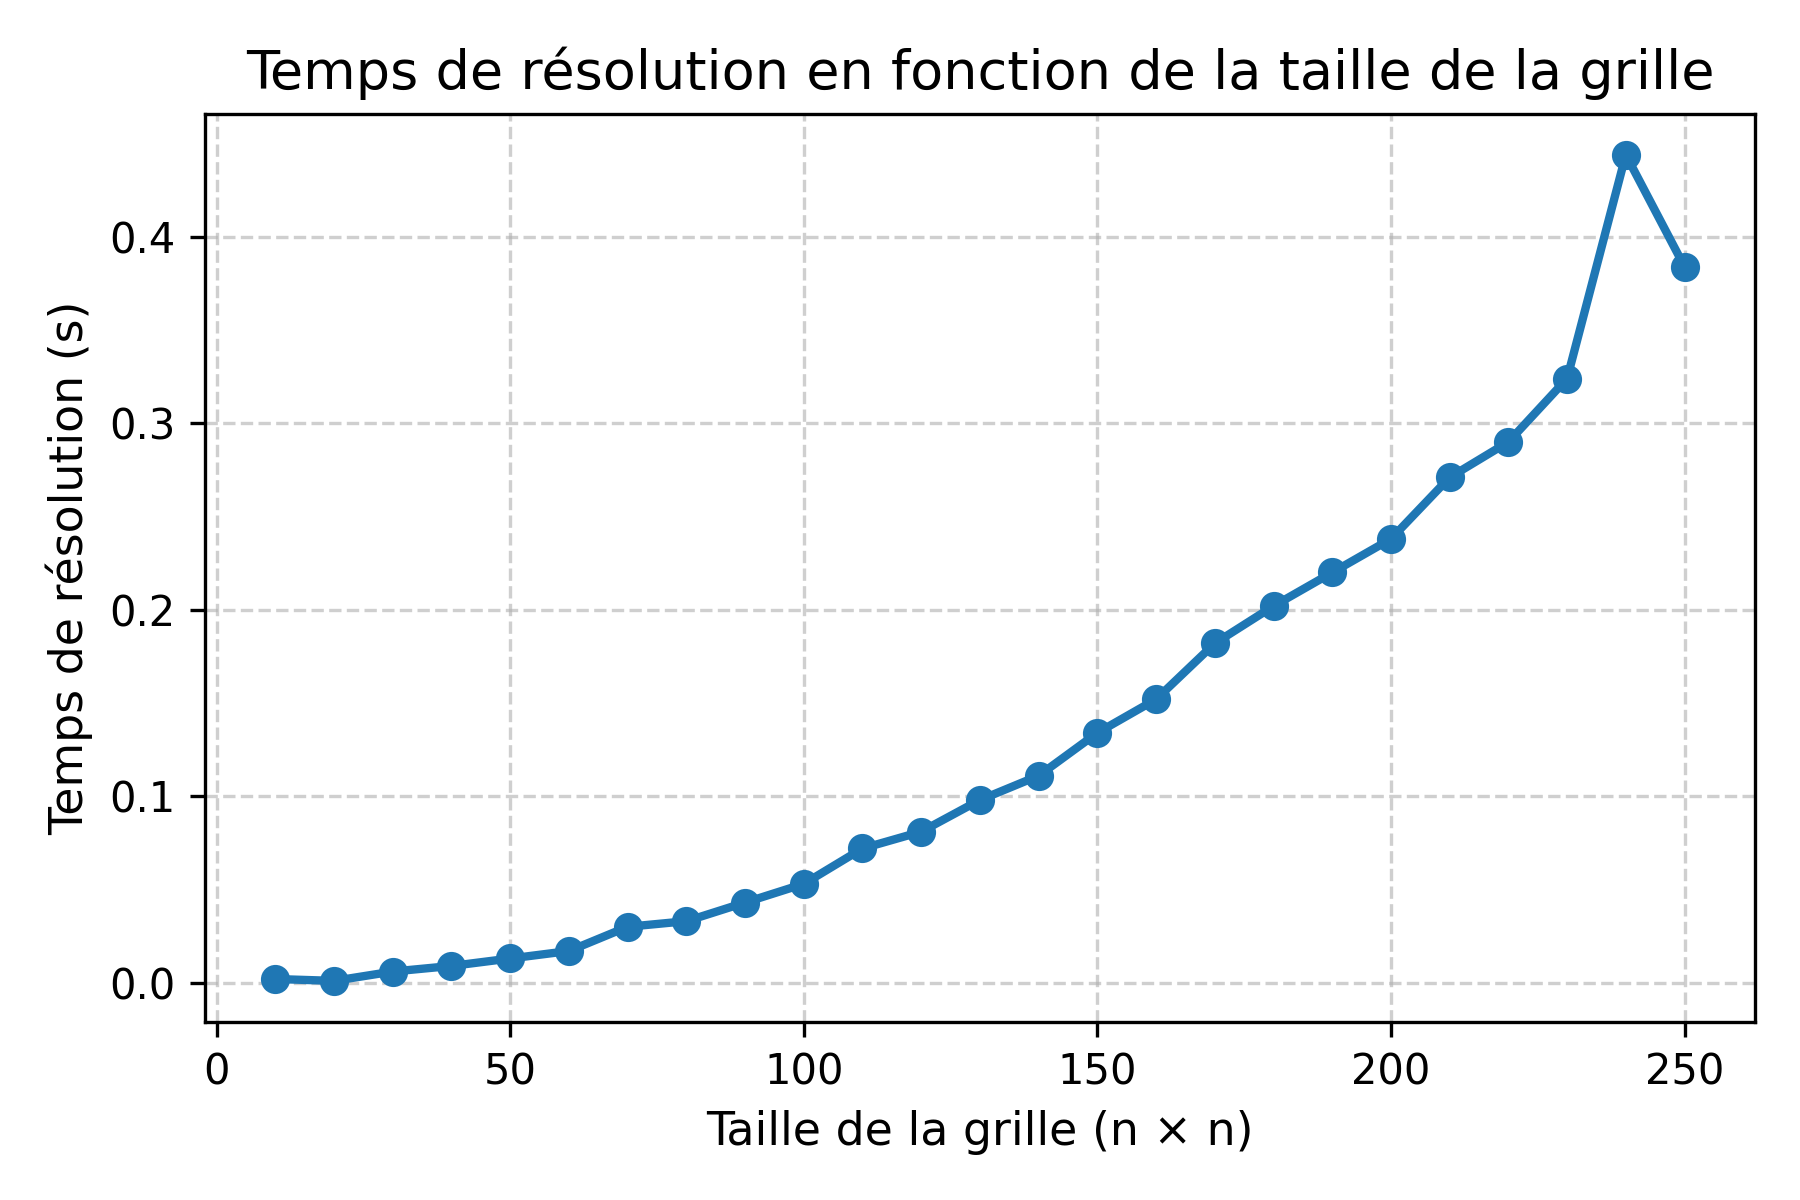
\includegraphics[width=0.7\textwidth]{figs/execution_time_P2_relaxed.png}
\end{figure}
Sans relaxation continue :
\begin{figure}[H]
  \centering
  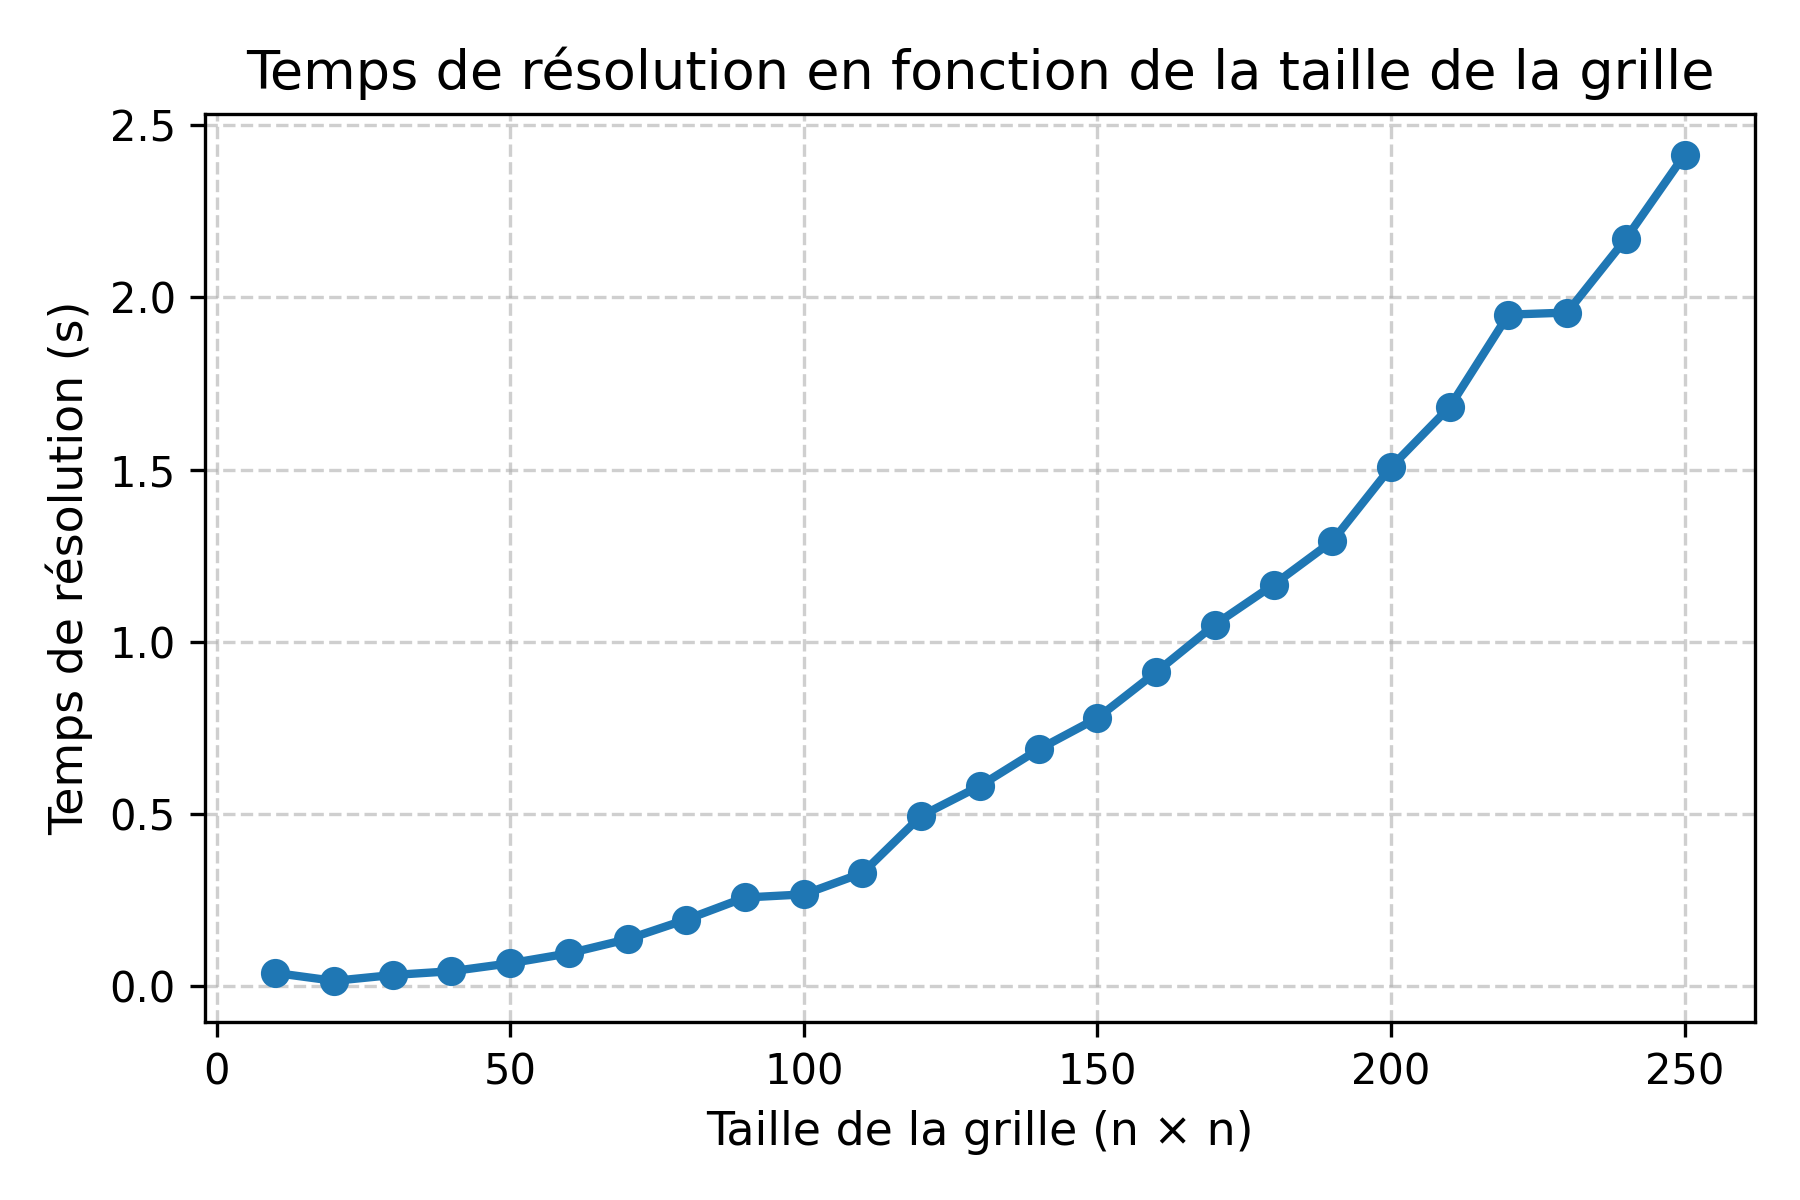
\includegraphics[width=0.7\textwidth]{figs/execution_time_P2_binary.png}
\end{figure}

On remarque que les modèles ont une évolution temporelle relativement similaire liés aux nombres de variables des modèles (quadratique dans les deux cas en la taille n de la grille).
La résolution de P2 sans contrainte sur les parcelles non coupées est remarquablement plus rapide. Il est aussi intéressant de remarquer que P1 sans la contrainte est significativment plus rapide que P1 avec ce qui semble capturé que cette contrainte fait basculer la complexité du problème comme on le voit dans le modèle P2.

\end{document}